%\documentclass[letterpaper, 10 pt, conference]{ieeeconf}
\documentclass[a4paper, 10pt, conference]{ieeeconf}      
                      
\IEEEoverridecommandlockouts                              
\overrideIEEEmargins

\usepackage[english]{babel}
\usepackage[utf8]{inputenc}
\usepackage{amsmath}
\usepackage{graphicx}
\usepackage[colorinlistoftodos]{todonotes}
\usepackage{float}
\usepackage{hyperref}
\usepackage{caption}  
\usepackage{enumitem}
\setlength{\parindent}{0cm}
\usepackage[toc,page]{appendix}
\usepackage{listings}
\usepackage{siunitx}
\usepackage{upgreek}
\usepackage{biblatex}
\usepackage{listings}
\usepackage{makecell, multirow}

\begin{document}
\title{\Huge \bf
ET4394 Final Project: \\
Dynamic Rate Control Algorithm for IEEE 802.11 WLAN
}
\author{
\begin{tabular}[t]{l@{\extracolsep{11em}}l@{\extracolsep{3em}}l} 
Niket Agrawal & Saumil Sachdeva \\
Student No: 4719514 & Student No: 4740998\\
Group WN3 & Group WN3\\
\end{tabular}
}
\maketitle
\thispagestyle{empty}
\pagestyle{empty}

\section{INTRODUCTION}

This report contains the description of the design, implementation and simulation of a closed loop control scheme based dynamic rate control algorithm for IEEE 802.11 WLAN. The proposed algorithm is built upon the rate control algorithm provided by Matlab in their WLAN toolbox [\ref{matlabcode}]. The proposed algorithm performs dynamic selection of Modulation and Coding Scheme (MCS) for each successive packet in order to achieve a high data rate and a low overall packet error rate.  


\section{Algorithm}
Two major changes feature in our proposed algorithm as compared to the algorithm provided in [\ref{matlabcode}]. 
\begin{enumerate}
    \item Dynamic adaptation of the SNR threshold values with each packet transmission
    \item Modification of the MCS selection and updating procedure
\end{enumerate}
%One is the dynamic adaptation of the SNR threshold values with each packet transmission and the other is the modification of the MCS selection and updating procedure. 
For the first, The algorithm in [\ref{matlabcode}] uses a fixed threshold of SNR values corresponding to each modulation and coding scheme (MCS). This mapping is used in the code to determine the MCS for a specific value of SNR by performing a simple look up and increasing/decreasing the MCS based on that. Since the SNR threshold values depend on the chipset of a device, we didn't choose the same set of values in our proposed algorithm, but rather dynamically improved the SNR threshold values with each packet transmission. For the initial set of values, we chose a corresponding minimum and maximum SNR value as obtained from [\ref{thresholds}].

For the second change, we believe choosing a range of SNR values for each MCS is much more logical rather than using just one fixed threshold value. By choosing a range of SNR's we can determine the MCS much more efficiently than using a fixed point. To implement this, two sets of threshold vectors are utilized in the algorithm. Lower threshold vector(LTs) contains the minimum value of SNR for each MCS (from 0 to 9), and the Higher threshold vector(HTs) contains the maximum value of SNR for each MCS. Another vector is initialized which holds the MCS values from 0 to 9. Three unique sets of lower and higher threshold vectors are used for channel widths of 40, 80 and 160 MHz. The algorithm chooses the right set of vectors to be used based on the channel width specified in the waveform configuration.
We discuss these changes in more detail in the following sub-sections.

\subsection{Logic to determine upper and lower MCS bounds}

The algorithm starts with the MCS initialized to 1. The first packet is transmitted with this MCS value. For subsequent packets, the MCS is determined based on the received SNR and bit error rate for the previous packets as per the algorithm mentioned in [\ref{referencepaper}].

Lower bound for the MCS is calculated by comparing the received SNR with the entries in the vector of low thresholds starting from index '9'. The index of the first entry which is smaller than the received SNR is recorded. Since the vector index and the MCS values are the same, the recorded index directly gives us the lower bound of the MCS.

Upper bound for the MCS is found by comparing the received SNR with the entries in the vector of High thresholds starting from index '0'. The index of the first entry which is greater than the received SNR is recorded. Since the vector index and the MCS values are the same, the recorded index directly gives us the higher bound of the MCS.  

\subsection{Determining MCS for subsequent packets}

Once the MCS bounds are calculated for a received SNR value, the MCS for the next transmission is determined by comparing the current value of the MCS (which was set for the previous packet) with these bounds. If the current MCS is higher than the upper bound, the MCS is decremented by 1. The below mentioned points summarizes the rationale behind this logic:

\begin{enumerate}
    \item The received SNR for the next packet is likely to be of the same order as the previous one so decreasing MCS by one is a valid approach to take.
    \item However, if the SNR for the next packet is indeed much higher than the previous value recorded, setting a lower MCS will not affect the throughput and bit error rate majorly since MCS is only decreased by '1'. Also, the bit error rate originating from this is handled for the next packet as the algorithm will sense the bit error rate and adjust the thresholds accordingly.
\end{enumerate}

And, if the magnitude of the current MCS value is lower than the lower bound, MCS is incremented by one. In case the current MCS is found to be equal to either of the lower or the upper bound, no changes are made to the MCS value. The rationale behind this approach is similar to the case of calculating lower bound as explained above.
By increasing and decreasing the MCS in such a way, we ensure that the MCS in every packet transmission tries to get to a value as close to the MCS bounds of the received SNR as possible.

\subsection{Dynamic adjustment of threshold values}

The algorithm has a mechanism to adjust the threshold values in the event of a bit error being detected after packet reception. It does this by using probe packets. For every received packet, the bit error rate is checked, if it is found to be a finite value and if the current MCS value is within close vicinity (+-1) of the MCS bound computed for the received SNR, two probe packets are sent, one with a MCS value one less than the current MCS and the second one with a MCS one more than the current MCS value. The bit error rate is checked again for the received packets corresponding to these two transmitted probe packets. If there's an improvement in the bit error rate, the threshold values are modified and updated in the threshold vectors in such a way that it ensures that if the same value of received SNR is seen next time, the MCS chosen will be the one which led to a lower bit error rate as per prior computation. 

This is done by setting the Higher threshold equal to the received SNR and Lower threshold as a fraction more than the Received SNR (in order to affect the condition check for computing lower threshold) if BER of the probe packet with MCS one less than the current MCS is better than the BER of the current packet. Similarly, if BER of the probe packet with MCS one more than the current MCS is better than the BER of the current packet then the Lower Threshold of the next index of the MCS of probe packet is set equal to the Received SNR and Higher Threshold of the index of MCS of probe packet equal to a little less than the Receieved SNR.
This is performed only when the current MCS is in the vicinity of the MCS bound calculated for the received SNR, so as to better mould the threshold vector as per the current channel conditions. Adjacent MCS values provide an opportunity to determine the optimal range of SNR threshold values. Since the algorithm continuously updates the thresholds depending on the channel conditions, it performs better with every iteration. The trend is plotted in Figure [\ref{Fig. 2}]

\subsection{Handling Empty Received SNR's}

There may be instances where the received PSDU is empty. The algorithm has a provision of handling such cases. This scenario was tested by modifying the input function in the Matlab sample code such that it overflows the specified SNR range a number of times. As a result, there are blank values seen in the estimated SNR fields upon reception. By checking the 'RxPSDU' field to be empty, this scenario is handled.

\section{Test setup}

An IEEE 802.11ac waveform consisting of a single VHT format packet is generated using wlanWaveformGenerator. The waveform is passed through a TGac channel and noise is added. The packet is synchronized and decoded to recover the PSDU. The algorithm was tested by varying different parameters in the waveform configuration and channel configuration like channel width for the former and noise profiles and receiver-transmitter distance for the latter.
Number of transmit antennas and spatial streams field in the waveform configuration were not modified for this project. 

\subsection{Simulating Dynamic conditions}

In this simulation 100 packets separated by a fixed idle time are transmitted through a TGac channel. The channel state is maintained throughout the simulation, therefore the channel evolves over time slowly [\ref{matlabcode}]. The resulting SNR measured at the receiver is slowly changed by this evolution [\ref{matlabcode}]. The algorithm in [\ref{matlabcode}] uses a parameter 'walkSNR'. Since the TGac channel changes very slowly over time, here an SNR variation at the receiver visible over a short simulation can be forced using this parameter to modify the noise power [\ref{matlabcode}].

Setting 'walkSNR' variable to true generates a varying SNR by randomly setting the noise power per packet during transmission [\ref{matlabcode}]. The SNR walks between 14-33 dB (using the amplitude and meanSNR variables) [\ref{matlabcode}].Setting 'walkSNR' variable to false fixes the noise power applied to the received waveform, so that channel variations are the main source of SNR changes at the receiver [\ref{matlabcode}].\\

\subsubsection{Rapidly varying SNR}
In order to further measure the performance of the algorithm for an input in which the SNR is varying rapidly, a random number generator based function is used as shown below:

\begin{lstlisting}[language=C]
randArray=5 + 33.*rand(100,1);
snrWalk = randArray(numPkt); 
\end{lstlisting}

where 'numPkt' is the $n^{\text{th}}$ packet. This generates SNR values in the range of 5-33 with random frequent fluctuations.

\section{Results}

\begin{enumerate}
    \item Figure \ref{Fig. 1} shows the comparison of the measured data rate for the proposed algorithm against the algorithm in [\ref{matlabcode}]. The data is collected for combinations of delay profiles and channel width. It is observed that the proposed algorithm provides better data rate than the algorithm in [\ref{matlabcode}] for channel width of 80MHz and in delay profiles D and F.
    
    \item Figure \ref{Fig. 2} shows the trend of the measured data rate of the proposed algorithm with each iteration of 100 packets. It is observed that overall, the data rate increases with every 100 packets. As mentioned earlier, the proposed algorithm updates the thresholds in case a bit error rate is detected, in order to adapt itself to the conditions and compute optimal SNR thresholds for each MCS. 
    
    \item Figure \ref{Fig. 3} shows the comparison of the measured data rate for the proposed algorithm against the algorithm in [\ref{matlabcode}] when the input SNR was generated purely using the random function generator as mentioned earlier. These measurements are done for N-LOS model delay profile D and channel width 40MHz. It is observed that the proposed algorithm provides marginally better data rate than the algorithm in [\ref{matlabcode}] for channel width of 80 MHz.
    
    \item Figure \ref{Fig. 4} shows the comparison of the measured packet error rate for the two algorithms. It is observed that the algorithm in [\ref{matlabcode}] offers a better packet error rate than our proposed algorithm (ran for one iteration)
    
    \item Figure \ref{Fig. 5} shows the trend of measured packet error rate of the proposed algorithm with each iteration. It is observed that overall, there is a decrease in the packet error rate with each iteration because of the way in which algorithm operates as explained earlier.
    
    \item The dynamic threshold adjustment feature in our algorithm contributes to an improved packet error rate. This observation is confirmed by measuring and comparing the results for two versions of our algorithm - one with the threshold feature adjustment feature enabled, and disabled in the other. The results are presented in table \ref{Table I}. The measurements were done at a channel width of 40MHz.
    
\end{enumerate}

\begin{figure}[h]
      	\centering
     	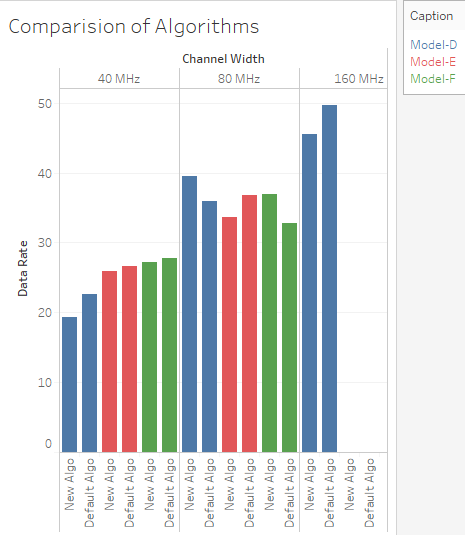
\includegraphics[scale=0.55]{AlgoComparision.png}
      	\caption{Data Rate Comparison}
      	\label{Fig. 1}
\end{figure}


\begin{figure}[h]
      	\centering
     	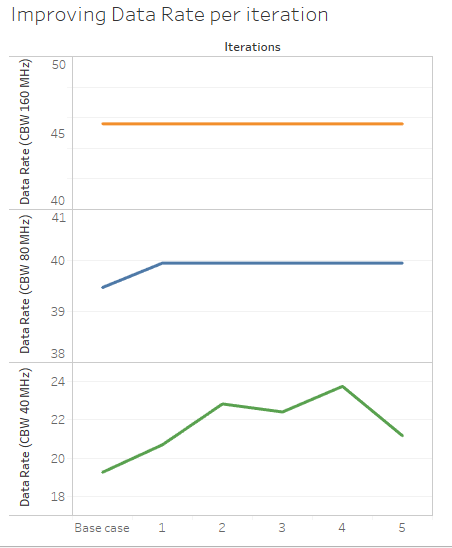
\includegraphics[scale=0.55]{DataRateVsIterations.png}
      	\caption{Data rate trend per iteration for proposed algorithm }
      	\label{Fig. 2}
\end{figure}

\begin{figure}[h]
      	\centering
     	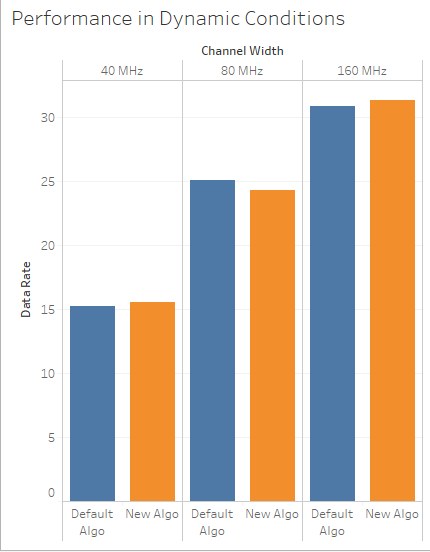
\includegraphics[scale=0.55]{DynamicConditions.png}
      	\caption{Data Rate comparison in dynamic conditions}
      	\label{Fig. 3}
\end{figure}

\begin{figure}[h]
      	\centering
     	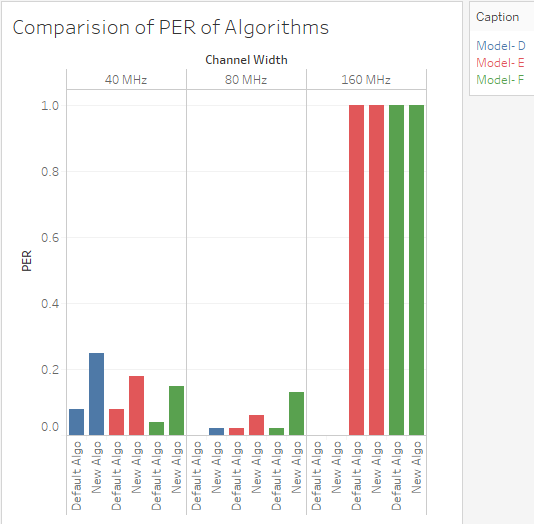
\includegraphics[scale=0.55]{PERAlgoComparision.png}
      	\caption{Packet Error Rate comparison}
      	\label{Fig. 4}
\end{figure}

\begin{figure}[h]
      	\centering
     	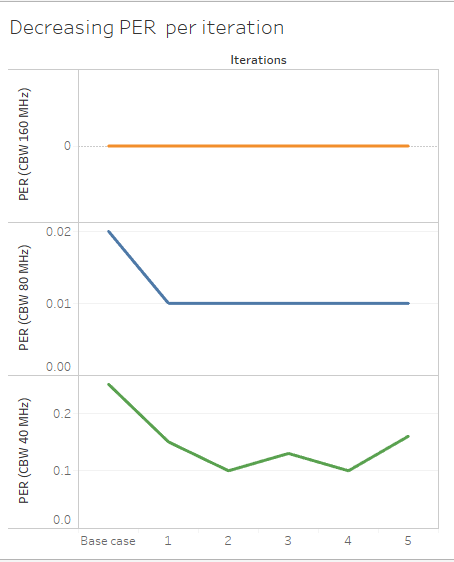
\includegraphics[scale=0.55]{PERvsIterations.png}
      	\caption{Packet Error rate per iteration}
      	\label{Fig. 5}
\end{figure}



\begin{table}[h]
\caption{Comparison of data Rate and packet error rate with and without dynamic threshold adjustment}
\label{Table I}
\centering
\begin{center}
%\begin{tabular}{|c|c|c|c|c|}
\begin{tabular}{|p{0.75cm}|p{1.30cm}|p{1.30cm}|p{1.30cm}|p{1.30cm}|}
  
\hline
Delay Profile  & Data rate with threshold adjustment & Packet error rate with threshold adjustment & Data rate without threshold adjustment & Packet error rate without threshold adjustment \\
\hline
D & 19.2578 & 0.25 & 18.7011 & 0.39 \\
\hline
E & 25.922 & 0.18 & 23.1133 & 0.3 \\
\hline
F & 27.2319 & 0.15 & 26.5207 & 0.18 \\

\hline
\end{tabular}
\end{center}
\end{table}




\section{Limitations and Future scope}

\begin{enumerate}
    \item Currently, the proposed algorithm doesn't support operation on channel width of 20MHz. The algorithm was designed keeping in mind that IEEE 802.11ac is associated with high throughput WANs operating at 5GHz. There simply isn't enough spectral bandwidth in the massively overused 2.4GHz band to allow for 802.11ac’s gigabit-level speeds. Channel bonding feature allows channel widths of 40MHz and 80 MHz (not as popular as 40MHz) to be commonly used and in some cases even 160 MHz. In order to enable support for 20 MHz, the algorithm needs to be restructured to ensure that a MCS of '9' is never used as its not available for 20MHz channel width. Also, in the current implementation, enabling support for 20MHz alone will contribute to addition of significant number of condition checks and reinforcements in the code which will not prove efficient.
    
    \item There is no provision of packets getting lost/dropped in the MATLAB's simulation environment used for this project. This limited us from not being able to drive the proposed rate control algorithm based on the packet loss which is an important metric while designing such algorithms.
    
    \item By sending probe packets, there is indeed an overhead in terms of bandwidth utilization, but this technique adds to the dynamics of the algorithm and helps it adapt to the surrounding conditions better.
\end{enumerate}

 

\section{CONCLUSION}

In this project we developed and simulated a closed loop control scheme based automatic rate control algorithm for IEEE 802.11ac WLAN. The proposed algorithm could adapt according to the conditions and gave a performance which was at par with the algorithm in [\ref{matlabcode}] with significant improvement especially at channel width of 80MHz. The algorithm in [\ref{matlabcode}] offered better packet error rate but the design is static unlike the dynamic SNR threshold adjustment in the proposed algorithm.  

\begin{thebibliography}{99}

\bibitem{referencepaper} \label{referencepaper}
  	Ivaylo Haratcherev, Koen Langendoen, Reginald Lagendijk, Henk Sips,Delft University of Technology, Delft, The Netherlands. MobiWac '04 Proceedings of the second international workshop on Mobility management \& wireless access protocols.
  	
\bibitem{matlabcode} \label{matlabcode}
https://nl.mathworks.com/help/wlan/examples/802-11-dynamic-rate-control-simulation.html

\bibitem{thresholds} \label{thresholds}
https://higher-frequency.blogspot.nl/2016/10/80211n-80211ac-data-rates-and-snr.html

\end{thebibliography}

\end{document}
